\documentclass[a4paper, 12pt]{article}
\usepackage{graphicx}
\usepackage{epstopdf}
\usepackage{float}
\usepackage{listings}
\usepackage[toc,page]{appendix}

\begin{document}
\begin{titlepage}
	\title{CSC469 Assignment 2}
	\author{Kats, Daniel \and Hong, Tony}
	\clearpage
	\maketitle
	\thispagestyle{empty}
\end{titlepage}

\section{Design}

Our design is a simplified version of Hoard, taking advantage of the fact that threads are never moved between processors.

\subsection{Data Structures}

\begin{itemize}
	\item A heap, one per processor, as well as a global heap (heap 0). This is implemented as an array of struct heap. We allocate a mutiple of the superblock-size which fits this data structure on initialization. We do this in order to align the memory in superblock-sized chunks.
	\item A global linked list of large blocks, which are large allocations. This is implemented as a linked list of struct largeblock. The  data for each entry is stored inside the memory location it references, so no initial memory is allocated.
	\item A per-heap linked list of reclaimed superblocks. The data is stored at the memory location it references, so no initial memory is allocated.
	\item A per-heap linked list of allocated superblocks, grouped by segment size (called seg-buckets). This is part of struct heap.
	\item Per-heap statistics of relative free-ness. This is part of struct heap.
\end{itemize}

The superblock structure, in depth:

\begin{itemize}
	\item The number of free spaces remaining
	\item The maximum possible number of free spaces
	\item The next and previous superblock in the linked list
	\item A linked list of free addresses
	\item A flag for whether this superblock is currently reclaimed or not
\end{itemize}

Superblock sizes are multiples of the page size (4KB), and segment sizes are powers of 2. The minimum allocation size is 64B, which we estimate to be the cache line size. We do this to prevent false-sharing.

The largeblock(large allocations) structure, in depth:

\begin{itemize}
	\item The next and previous superblock in the linked list
\end{itemize}

\subsection{Locks}

\begin{itemize}
	\item lock around mem\_sbrk syscall, when creating new superblocks, or new large blocks
	\item lock for each heap, when traversing per-heap freelist or superblocks in one of the heap's segment buckets
	\item lock for the large-list, for traversal
\end{itemize}

\subsection{General Algorithm and Overview}

\subsubsection{mm\_malloc}

On an allocation, we compare the size requested to the maximum segment size (which is half the superblock size). If it is larger, then we consider this a large allocation. If not, we allocate 'normally'.

For a large allocation:

\begin{itemize}
	\item Allocate a multiple of the superblock size, such that we can fit in header information and the data size
	\item Store header information in the first few bytes of the large block
	\item Return a pointer to the area immediately following the header data
\end{itemize}

For a small allocation:

\begin{itemize}
	\item Identify the correct heap by using sched\_getcpu() system call
	\item Identify the correct segment size for the allocation, which is the smallest power of 2 larger than the requested size
	\item Iterate over the free list of each superblock in the corresponding seg-bucket, looking for a non-empty freelist. If found, remove the head of the freelist, and return this address.
	\item Check the reclaimed superblocks list for this heap. If the list is not empty, pop the first superblock and initialize it to the proper segment size. The first free node from that superblock's freelist is removed and returned.
	\item Check the reclaimed superblocks list for heap 0. If the list is not empty, pop the first one and initialize it to the proper segment size. It is then put into the seg-bucket of this heap, and the first free node from that superblock's freelist is removed and returned.
	\item If all else fails, we allocate a new superblock. We reserve the correct number of segments at the top for header information, and the rest are turned into free nodes in the superblock's freelist. Remove and return the first node in the freelist.
    \item We then update the heap's statistics.
\end{itemize}

We store the struct superblock and the struct largeblock in the header of the allocated memory. The superblock header data will be stored in a region of a multiple of the segment size, for easier calculation.

\subsubsection{mm\_free}

We try to determine if the address belongs to a large allocation or a small allocation. We traverse the largelist, and if we do not find corresponding memory, it is a small allocation.

For a large deallocation:

\begin{itemize}
	\item Remove the relevant block from the largelist
	\item Break up the block into superblocks, and add them to heap 0's freelist of superblocks
\end{itemize}

For a small deallocation:

\begin{itemize}
	\item Identify the address of the superblock to which the address belongs, by flooring it appropriately (all superblocks are SB-size aligned)
	\item Add the segment to the superblock's freelist.
	\item Read the header information of the superblock, and if the superblock is now empty, remove it from all relevant data structures. The superblock is then added to the relevant heap's list of free superblocks.
	\item We then update the heap's statistics. If they match our thresholds, and the current heap has free superblocks, then move a free superblock from the currrent heap to heap 0's list of free superblocks.
\end{itemize}

\section{Optimizations}

\subsection{Included}


When a heap needs to allocate a new superblock, it needs to get the sbrk\_lock. This means that this thread will be holding two important locks, and potentially delaying other threads' operations. To address this, we programmed malloc to temporary release the lock while allocating new superblocks, and we observed a slight improvement in performance.

We implemented a test-and-test-and-set -like heuristic for lock acquisition in various locations. Here we are concerned about performance more than blow-up. For instance, in malloc, if we want to check the free list of heap 0, we first check if the free list is NULL before acquiring the lock to heap 0, and we check it again afterwards to make sure it is consistent. This is in general much faster than waiting for the lock to become available, and then discovering that it is already NULL. This improved the overall performance of the program, at the cost of some minor memory blow-up. The first NULL check is meant to give us a general idea of the state of heap 0's freelist, and is not meant to be completely accurate.

\subsection{Excluded, but tried}

We have tried implementing seg buckets for heap 0. This means that when no free nodes are available for a heap to move to heap 0, it will move a partially free node from one of its seg-buckets to the corresponding seg-bucket of heap 0. This allows other heaps to use that superblock for their allocation even though there are still allcoations belonging to the original heap. This implmentation led to much slower performance due to the extra overhead of finding the optimal(least occupied) superblock to evict. So we scrapped it in favor of better performance, at the cost of potentially increasing our blow-up.

\subsection{Future Work}

To find a free block, we current scan through all the superblocks in a given segment bucket and heap. However, if the superblocks were sorted such that either: the first superblock in the linked list has a free space, or NONE of the superblocks in the linked list have space. This would cut down on the worst-case traversal of this list from $O(n)$ to $O(1)$. The proposed way to do this is to move superblocks occasionally on free and malloc in the following way:

\begin{itemize}
	\item If we have just allocated the last free space in a superblock, move it to the back of the linked list
	\item If we have just created free space in a superblock, move it to the front of the linked list
\end{itemize}

This ensures that the first item in each linked list obeys the property above. Unfortunately, while trying to implement this, we ran into some bugs which we were unable to fix in time for the deadline, so we removed this feature altogether.

The above idea could also be implemented by implementing per-seg-bucket free-counters.

Another idea is to implement more fine-grained locking over the heaps. Since we are altering at most the sb\_freelist and a single seg-bucket per alloc/free, we could lock down those two areas, leaving the other areas of the heap unlocked to traversal.

\section{Results}

Below are graphs similar to those generated by the various Perl graphing scripts. Our graphs are generated from the same data file which the graphing scripts create, but process the data using Python rather than gnuplot to get \textbf{beautiful colors}.

The results for libc and kheap were taken from our early runs, as the later runs did not give back results for libc and kheap. Since we did not alter either of those two algorithms, we contend the results are valid.

We ran our allocator on CDF's wolf as well, giving us similar results across all the benchmarks. We do not include these graphs for brevity.

\vfill
\begin{center}
	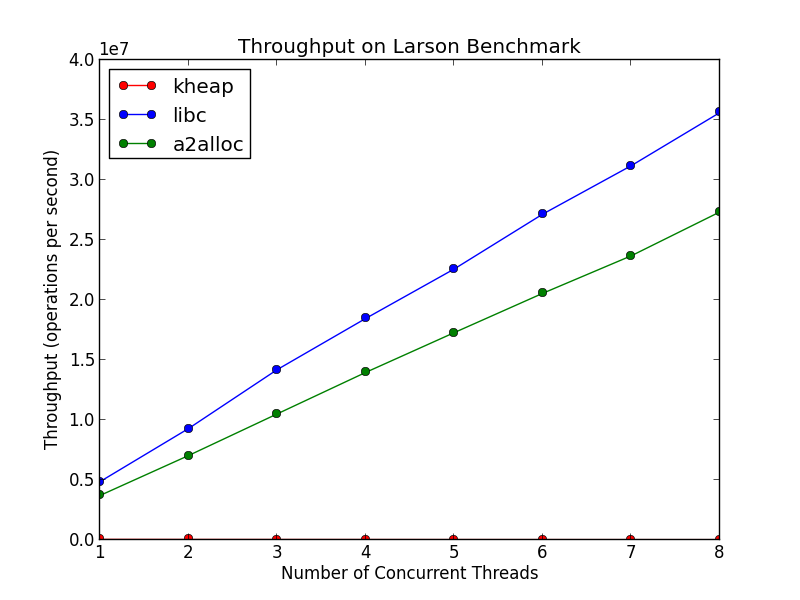
\includegraphics[width=6.0 in]{larson_throughput.png}
\end{center}
\vfill

\vfill
\begin{center}
	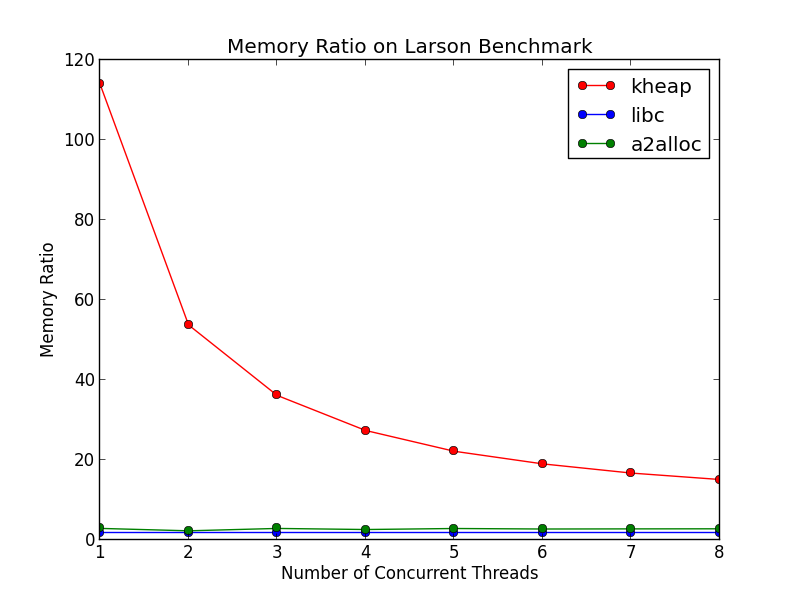
\includegraphics[width=6.0 in]{larson_memory.png}
\end{center}
\vfill

\vfill
\begin{center}
	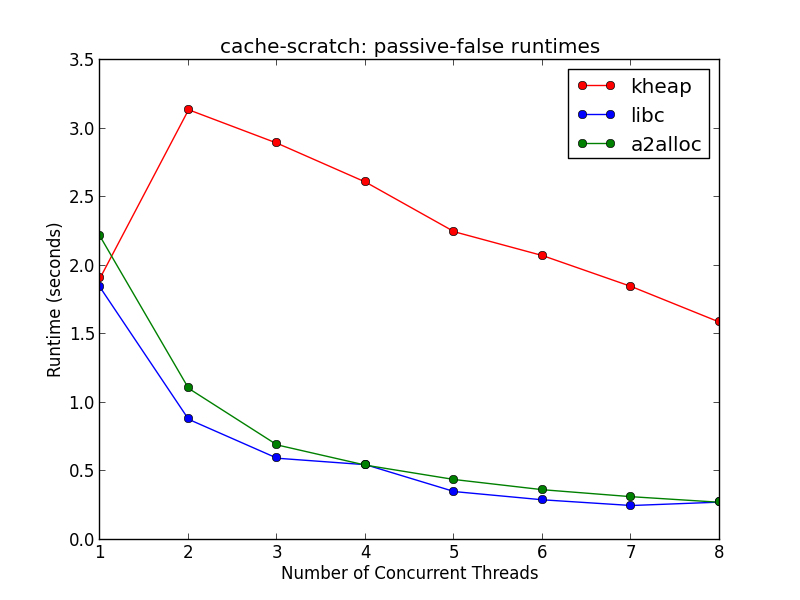
\includegraphics[width=6.0 in]{cache-scratch.png}
\end{center}
\vfill

\vfill
\begin{center}
	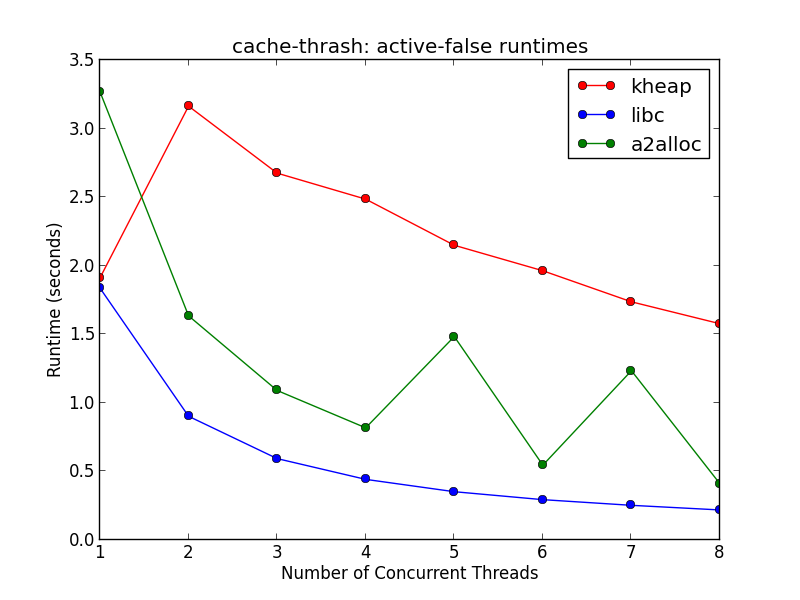
\includegraphics[width=6.0 in]{cache-thrash.png}
\end{center}
\vfill

\vfill
\begin{center}
	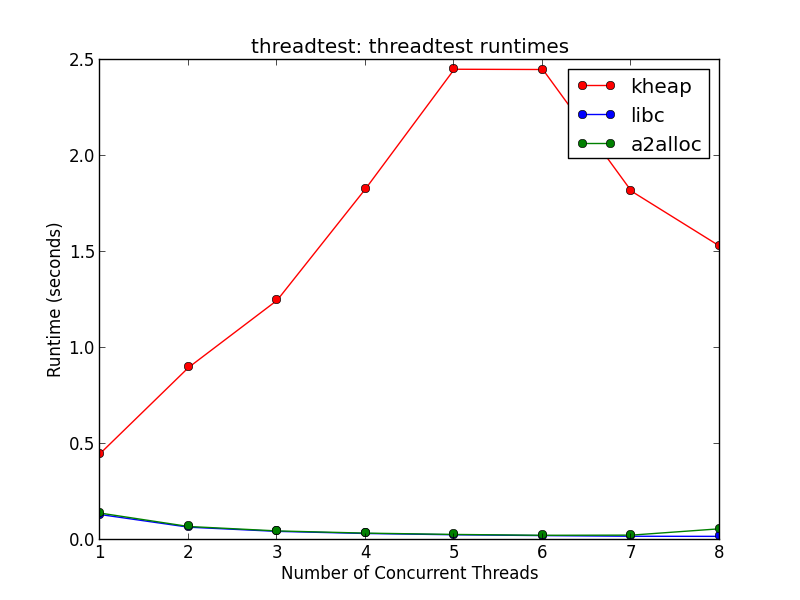
\includegraphics[width=6.0 in]{threadtest.png}
\end{center}
\vfill

\section{Analysis}
In all of the benchmarks, our memory allocator mimics libc's performance, and it out-performs kheap in every aspect.

\subsection{Larson}
We observed an increase in throughput as more processors were added, consistent with our goal of a scalable allocator. Unfortunately, the rate of increase is less than that of libc. Libc's "scalability factor" (rate of throughput increase) is approximately 4.29 Million operations per second per core, whereas our rate of increase is 3.00 Million operations per second per core. We speculate that the extra overhead of maintaining the heap is what is causing this discrepancy.

In addition, we could improve the scalability by adding more fine-grained locking, as we talk about in the future work section.

In terms of the memory ratio on this benchmark, we keep a relatively constant ratio, which is consistent with the theory of hard. Our blowup is approximately 5.1, because of small allocations within the benchmark - we allocate a minimum of 64B because this is the cache line size. If the average requested is 12B, then the blowup will be approximately 5, which is what we have. We contend that real-life allocations would be higher than 12B on average, so the blowup would be much smaller.

\subsection{Cache-Scratch and Cache Thrash}
Since heaps would only return superblock to heap 0 when it is empty, and each thread is assigned to a specific heap, we can ensure that the amount of false sharing is minimal. This is consistent with our findings, since runtime of our allocator is only slightly higher than libc's.

Our passive false sharing performance is quite a bit better than our active false-sharing performance. We believe that this has to do with optimized libc performance and more fine-grained locking in libc. We are not sure why 7 threads cause particular contention which break the downward trend, but we see this result across multiple runs.

We believe the slight increase above libc is based in small runtime improvements present in libc, rather than some major oversight on our part.

\subsection{Threadtest}

The threadtest graph shows that a2alloc is approximately as scalable as libc. This is consistent with the throughput graph we had in Larson, as well as the goal of the assignment.

\begin{thebibliography}{1}
	\bibitem{hoard} Berger et. al. {\em Hoard: A Scalable Memory Allocator for Multithreaded Applications} 2000.
\end{thebibliography}

\end{document}
